\subsection{Evaluation of \Hammer}
\label{minjia_subsec:iqan-eval}

\Hammer offers significant speedups than two state-of-the-art graph-based ANNS, NSG~\cite{NSGGithub,nsg} and HNSW~\cite{HNSWGithub,hnsw} over several public datasets, including SIFT1M (128D), GIST1M (960D), DEEP10M (96D), DEEP100M (96D), and SIFT100M (128D). We measure the latency and \emph{Recall@100} (R@100), which measures the accuracy of finding the top-100 nearest neighbors for every query.
We conduct our experiments on a workstation with Xeon Gold 6138 (2.00 GHz) with 20 cores and 128 GB DRAM (\emph{Skylake} for short). 

Fig.~\ref{minjia_fig:eval-latency} compares the latency of HNSW, NSG, and \Hammer on Skylake. NSG and HNSW use their sequential search algorithm, whereas \Hammer uses 16 threads on Skylake. Across all five datasets, \emph{\Hammer consistently provides latency speedups over existing sequential-based approaches NSG and HNSW over a wide range of recall targets. }
In particular, the speedups from \Hammer increase as the recall target moves to the high accuracy regime (e.g., from 0.90 to 0.999).
Notably, \Hammer achieves up to $12.9\times$ speedups over NSG on DEEP100M on Skylake, obtaining an incredibly low latency of $<$5ms or $<$3ms at the recall target 0.999 by leveraging aggregated multi-core computation and memory bandwidth resources. This enables vector search with very high accuracy on large-scale graphs, even in extremely interactive online applications. 

\Hammer achieves significant latency speedups mainly for three reasons. First, \Hammer's path-wise parallelism effectively reduces the iteration depths, making the sequential dependencies no longer a major bottleneck. This is particularly critical for a large graph (e.g., DEEP100M) and high recall (e.g., 0.999) as seen in Section~\ref{minjia_subsec:iqan-design} that the iteration depths increase significantly as we either scale the graph size or increase the recall targets. 
Second, the reduced iteration depths do not come at the cost of many redundant computations as \Hammer leverages staged expansion to effectively avoid redundant computations from doing path-wise parallelism. Third, \Hammer significantly reduces the synchronization overhead through redundancy-aware synchronization.
It is also worth mentioning that \Hammer achieves excellent speedups as we increase the dimensionality of the embedding vectors. \Hammer achieves up to $24.9\times$ speedups over HNSW on GIST1M on Skylake. This is higher than the speedups we get on a dataset with a similar scale but much smaller dimensionality (e.g., SIFT1M). \Hammer is able to achieve better speedups on higher dimensional vectors because as the vector dimension increases, the amount of computation workload for the pair-wise distance computation also increases, which allows \Hammer to benefit more from parallel computing. 

\begin{figure*}
    \centering
    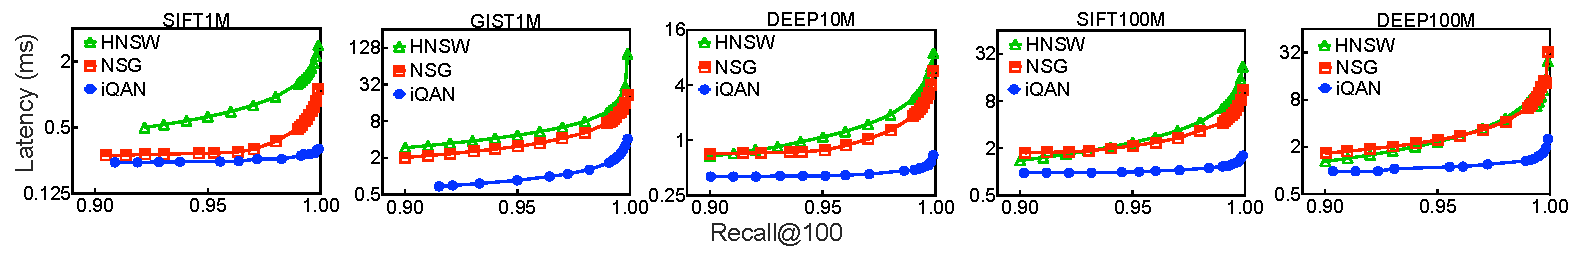
\includegraphics[width=0.98\textwidth]{submissions/Minjia2023/figures/eva_runtime_Skylake}
    \caption[Study of Latency]{Latency comparison among HNSW, NSG, and \Hammer on  Skylake (16T).}
    \label{minjia_fig:eval-latency}
    % \vspace{-1em}
\end{figure*}

\textbf{Comparison with DiskANN.} Fig.~\ref{minjia_fig:eva_runtime_recall-1_KNL} compares the latency of DiskANN~\cite{subramanya32diskann} (using 1 thread with its in-memory index) and \Hammer (using 32 threads) for \emph{Recall@1} targets. 
For building its indices of datasets SIFT1M and GIST1M, DiskANN uses $L=125$, $R=70$, $\alpha = 2$, which are the same setting as shown in its paper. For DEEP10M, DiskANN uses $L=100$, $R=100$, $\alpha=1.2$. 
Fig.~\ref{minjia_fig:eva_runtime_recall-1_KNL} shows that \Hammer achieves significant latency speedups over DiskANN, especially for the high recall regime. For example, for recall target 0.999, \Hammer has about $180.5\times$ average speedup on DiskANN among these three datasets.

\begin{figure}[t]
\begin{minipage}[t]{0.55\textwidth}
    \centering
    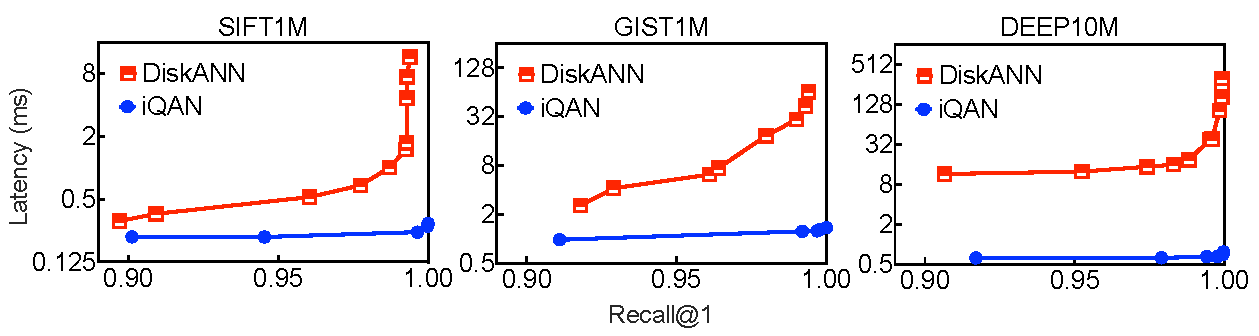
\includegraphics[width=0.98\textwidth]{submissions/Minjia2023/figures/eva_runtime_recall-1_KNL}
    \caption[Recall@1 Latency]{Recall@1 latency of DiskANN and \Hammer.
    }
    \label{minjia_fig:eva_runtime_recall-1_KNL}
\end{minipage}
\hfill
\begin{minipage}[t]{0.42\textwidth}
    \centering
    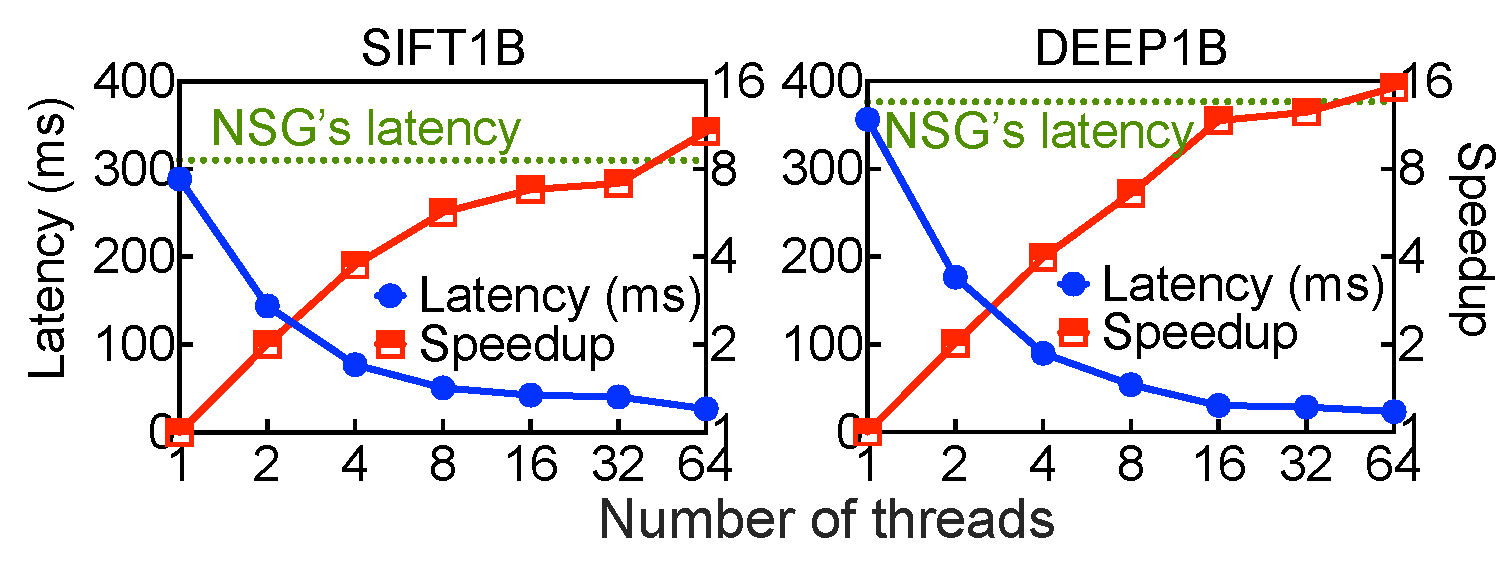
\includegraphics[width=0.98\textwidth]{submissions/Minjia2023/figures/eva_sift1b_deep1b_latency}
    \caption[Latency for 1B datasets]{Performance comparison of \Hammer and NSG on two billion-scale datasets SIFT1B (\texttt{bigann}) and DEEP1B. 
        }
    \label{minjia_fig:eva_sift1b_deep1b_latency}
\end{minipage}
\end{figure}


\textbf{Scaling to billion points.}
This experiment is conducted on a machine with a 1.5 TB memory.
It is worth mentioning that even 1.5 TB of memory is not enough to build a 100-NN graph with one billion data vectors. Therefore, we limit the out-degree of NSG
when generating the corresponding NSG index so that the index construction can finish in a reasonable amount of time (e.g.,<10 days). We also note that this is the first time to evaluate an NSG graph at a billion scale as the maximum graph prior work such as NSG evaluated contained less than 100M data points. Fig.~\ref{minjia_fig:eva_sift1b_deep1b_latency} compares the latency of \Hammer and NSG. \Hammer uses up to 64 threads, and the recall target is 0.9. 
When using 64 threads, \Hammer follows the trend of scalability we observed as we increase the graph size and outperform NSG with $11.5\times$ and $16.0\times$ speedup for SIFT1B and DEEP1B, respectively, confirming the excellent scalability of \Hammer on large-scale graphs again. 






